\section{Pendahuluan}
Dengan membuat tabel berfungsi agar aplikasi terhubung dengan database, dalam buku ini kita akan membuat beberapa tabel yang saling berelasi, tabel ini mempunyai atribut yang dimiliki pada data yang mengacu pada aplikasi.

\subsection{Definisi Database Menurut Para Ahli}
Kemampuan basis data Oracle dapat bekerja pada banyak platform merupakan salah satu  fasilitas  yang dimanfaatkan untuk  menyimpan data dengan membuat sub routine sehinggadalam  melakukan eksekusi data menjadi  cepat \cite{pemanfaatandatabase2018}.

\par Oracle merupakan sebuah sistem manajemen basis data yang dikenal memiliki fitur dan kecanggihan yang membuat pengelolaan basis data menjadi efisien dan efektif. Namun perancangan basis data yang diterapkan pada suatu sistem manajemen basis data tidak kalah pentingnya. Perancangan basis data yang baik akan mempermudah implementasi aplikasi serta mengoptimalkan kinerja dari sistem manajemen basis data itu sendiri\cite{perancanganDB2013}.

\par Pengolahan data untuk menghasilkan informasi secara terkomputerisasi, merupakan sarana yang sangat dibutuhkan saat ini pada berbagai jenis usaha, karena informasi mampudisajikan dalam waktu yang cepat dan akurat. Informasi yang mampu disajikan dengancepat dan akurat mampu menghasilkan pengambilan keputusan yang cepat dan efektif\cite{jurnalDB2011}.

\section{Siapkan Tabel}
Dalam pembuatan tabel kita siapkan 7 tabel untuk mengelola aplikasi absensi pada buku ini yaitu :
\begin{itemize}
    \item[1]JABATAN\_ORMAWA
            \begin{itemize}
                \item KODE\_JABATAN (NUMBER) PK
                \item JABATAN (VARCHAR2(50))
            \end{itemize}
    \item[2]JURUSAN
            \begin{itemize}
                \item KODE\_JURUSAN (NUMBER) PK
                \item NAMA\_JURUSAN (VARCHAR2(255))
            \end{itemize}
    \item[3]ORMAWA
            \begin{itemize}
                \item KODE\_ORMAWA (VARCHAR2(255)) PK
                \item NAMA\_ORMAWA (VARCHAR2(255))
            \end{itemize}
    \item[4]RUANGAN
            \begin{itemize}
                \item ID\_RUANGAN (NUMBER) PK
                \item JENIS\_RUANGAN (VARCHAR2(255))
            \end{itemize}
    \item[5]STAFF\_BAAK
            \begin{itemize}
                \item NIK (NUMBER) PK
                \item NAMA\_STAFF (VARCHAR2(255))
                \item NO\_TELP (VARCHAR2(20))
                \item JABATAN (VARCHAR2(30))
            \end{itemize}
    \item[6]MAHASISWA
            \begin{itemize}
                \item NPM (NUMBER) PK
                \item NAMA (VARCHAR2(255))
                \item KELAS (VARCHAR2(255))
                \item KODE\_ORMAWA (VARCHAR2(255)) FK
                \item NO\_TELP\_MHS (VARCHAR2(14))
                \item KODE\_JURUSAN (NUMBER) FK
                \item KODE\_JABATAN (NUMBER) FK
            \end{itemize}
    \item[7]PEMINJAMAN\_RUANGAN
            \begin{itemize}
                \item ID\_PEMINJAMAN (NUMBER)
                \item NPM (NUMBER) FK
                \item ID\_RUANGAN (NUMBER) FK
                \item NIK (NUMBER) FK
                \item TANGGAL (DATE)
                \item JAM\_AWAL (VARCHAR2(4000))
                \item JAM\_AKHIR (VARCHAR2(4000))
                \item STATUS\_PEMINJAMAN (VARCHAR2(4000))
            \end{itemize}
    \par KETERANGAN :
            \begin{itemize}
                \item NUMBER = Tipe Data Sebagai NOMER/ANGKA
                \item DATE = Tipe Data Sebagai TANGGAL
                \item VARCHAR2 = Tipe Data Sebagai NOMER/ANGKA/SIMBOL
                \item PK = Primary Key, Kunci Utama/Unik Untuk Merelasikan Antar Tabel
                \item FK = Foreign Key, Kunci Kedua/Kunci Asing untuk merelasikan dari kunci unik/Primary Key
            \end{itemize}
    
        \begin{figure}
        \par Lalu merelasikannya seperti Gambar berikut :
        \begin{center}
        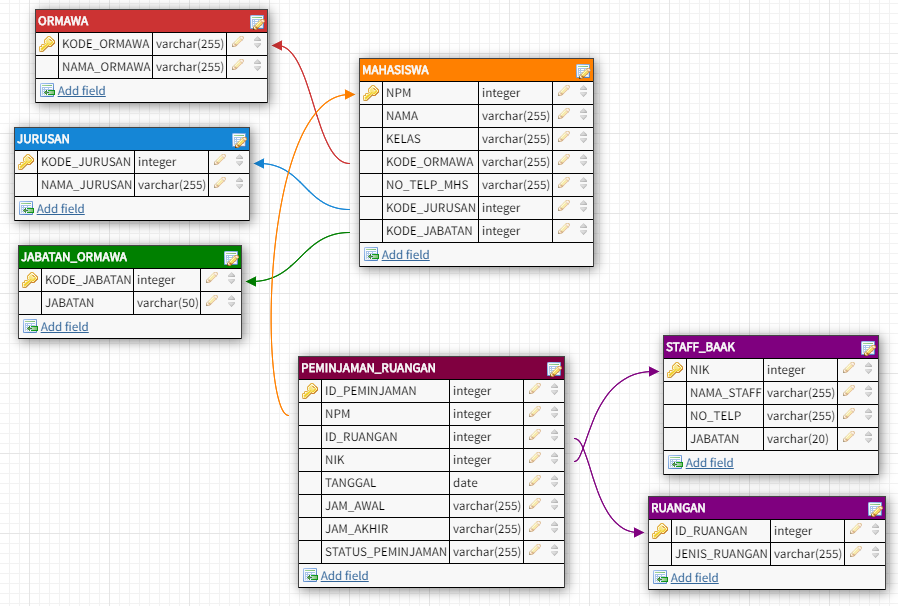
\includegraphics[scale=0.45]{figures/TABEL.png}
        \caption{\textit{TABEL DATABASE}}
        \end{center}
        \end{figure}
\end{itemize}